% Template for Cogsci submission with R Markdown

% Stuff changed from original Markdown PLOS Template
\documentclass[10pt, letterpaper]{article}

\usepackage{cogsci}
\usepackage{pslatex}
\usepackage{float}
\usepackage{caption}

% amsmath package, useful for mathematical formulas
\usepackage{amsmath}

% amssymb package, useful for mathematical symbols
\usepackage{amssymb}

% hyperref package, useful for hyperlinks
\usepackage{hyperref}

% graphicx package, useful for including eps and pdf graphics
% include graphics with the command \includegraphics
\usepackage{graphicx}

% Sweave(-like)
\usepackage{fancyvrb}
\DefineVerbatimEnvironment{Sinput}{Verbatim}{fontshape=sl}
\DefineVerbatimEnvironment{Soutput}{Verbatim}{}
\DefineVerbatimEnvironment{Scode}{Verbatim}{fontshape=sl}
\newenvironment{Schunk}{}{}
\DefineVerbatimEnvironment{Code}{Verbatim}{}
\DefineVerbatimEnvironment{CodeInput}{Verbatim}{fontshape=sl}
\DefineVerbatimEnvironment{CodeOutput}{Verbatim}{}
\newenvironment{CodeChunk}{}{}

% cite package, to clean up citations in the main text. Do not remove.
\usepackage{apacite}

% KM added 1/4/18 to allow control of blind submission


\usepackage{color}

% Use doublespacing - comment out for single spacing
%\usepackage{setspace}
%\doublespacing


% % Text layout
% \topmargin 0.0cm
% \oddsidemargin 0.5cm
% \evensidemargin 0.5cm
% \textwidth 16cm
% \textheight 21cm

\title{Analyzing contingent interactions in R with \texttt{chattr}}


\author{{\large \bf Marisa Casillas (mcasillas@uchicago.edu)} \\ Comparative Human Development, 1101 E. 58th St. \\ Chicago, IL 60637 USA \AND {\large \bf Camila Scaff (camila.scaff@iem.uzh.ch)} \\ Institute of Evolutionary Medicine, University of Zurich \\ Zurich, Switzerland CH-8057}


\begin{document}

\maketitle

\begin{abstract}
The \texttt{chattr} R package enables users to easily detect and
describe temporal contingencies in pre-annotated interactional data.
Temporal contingency analysis is ubiquitous across signal system
research, including human and non-human animal communication. Current
approaches require manual evaluation (i.e., do not scale up), are
proprietary/over-specialized (i.e., have limited utility), or are
constructed ad-hoc per study (i.e., are variable in construct).
\texttt{Chattr}'s theoretically motivated, customizable, and open source
code provides a set of core functions that allow users to quickly and
automatically extract contingency information in data already annotated
for interactant activity (via manual or automated annotation). We
demonstrate the use of \texttt{chattr} by testing predictions about
turn-taking behavior in three language development corpora. We find that
the package effectively recovers documented variation in linguistic
input given both manual and automatically created speech annotations and
note future directions for package development key to its use across
multiple research domains.

\textbf{Keywords:}
Contingency; interaction; turn taking; LENA; communication; R; software.
\end{abstract}

\hypertarget{introduction}{%
\section{Introduction}\label{introduction}}

\texttt{Chattr} is an R package that facilitates the detection and
analysis of temporally contingent interactions in pre-annotated data
(URL redacted).\footnote{All documentation and scripts are available at
  the URL; the fully packaged version will be available before May 2021.}
Its utility extends across studies of human interaction, non-human
animal communication, and contingencies within multi-modal signals.
Despite significant common conceptual ground between these domains,
definitions of contingency phenomena and implementations of contingency
detection remain inconsistent, foregoing critical opportunities for the
accumulation of shared construct validity. Such divergences are partly
due to a lack of flexible contingency analysis tools: existing systems
are either constructed ad-hoc, limited in use, or proprietary.
\texttt{Chattr} improves this situation by: (1) taking inspiration from
conversation analysis, psycholinguistics, and language development to
provide theoretically sound, but customizable measurements of temporally
contingent interaction at scale and (2) accepting a handful of generic
formats as input, opening up its analytical framework to broad
application (e.g., child language input, multi-party conversation,
non-human animal signaling, event contingencies, etc.). Here we review
\texttt{chattr}'s theoretical basis, describe the package's core
functions, and demonstrate its use in three existing datasets.

\begin{CodeChunk}
\begin{figure*}[h]

{\centering 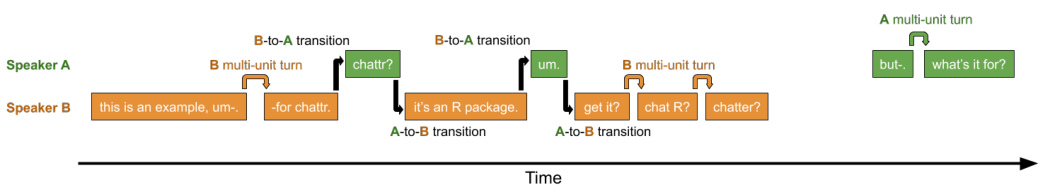
\includegraphics{figs/minisequence-1} 

}

\caption[An example of a brief dyadic interaction between two English speakers]{An example of a brief dyadic interaction between two English speakers: A (green) and B (orange). The producers here use both single- and multi-unit turns. There are 6 turns (3 from each producer), 4 turn transitions (two each from B to A and vice versa; black arrows), and one interactional sequence (the contiguous block of producer continuation/transition marked with green/orange arrows; the other turn ('but-. what's it for?') has no transitions and so is not in an interactional sequence).}\label{fig:minisequence}
\end{figure*}
\end{CodeChunk}

\hypertarget{contingent-interaction}{%
\subsection{Contingent interaction}\label{contingent-interaction}}

Joint coordination of action by two or more agents usually involves
temporal contingencies. Whether we are making music with others,
crossing a busy intersection, or chatting with a friend, the timing of
our contributions to a coordinated event is crucial to its success.
Optimal strategies for coordination often involve turn taking, that is:
typically, only one interactant makes their contribution at a time, and
decisions about who contributes when can be determined flexibly (as in
conversation) or in a pre-defined manner (as in a debate). This
sequential structure enables interactants to adapt each contribution
such that it relevantly progresses the joint activity and to initiate
unplanned sub-sequences (e.g., repairing misunderstandings) without
breaking progress toward the larger goal.

Turn-taking (and similar) interactions are essential for communication
across the animal kingdom (Fröhlich et al., 2016; Pika, Wilkinson,
Kendrick, \& Vernes, 2018), as well as AI systems interacting with human
users. In humans, turn-taking interactions may be the only reliable
source of language universals (Levinson, 2019). Traditionally, these
kinds of interactional contingencies have been studied using careful
inspection and analysis, both qualitative and quantitative, of manual
measurements from video and audio recordings. However, recent advances
in recording devices and automated annotation software (e.g., for voice
detection) have created a growing need for new analytical approaches
that can capitalize on very large, but relatively noisy datasets that
cannot feasibly be assessed by hand.

\hypertarget{current-contingency-detection-approaches-and-their-limitations}{%
\subsection{Current contingency detection approaches (and their
limitations)}\label{current-contingency-detection-approaches-and-their-limitations}}

At present, the most widely used tool for automated contingency analysis
of human interaction is the LENA system (Greenwood, Thiemann-Bourque,
Walker, Buzhardt, \& Gilkerson, 2011), which was built for use with
young children, but has also been employed to capture adult language
environments (e.g., Rodríguez-Arauz, Ramírez-Esparza, García-Sierra,
Ikizer, \& Fernández-Gómez, 2019). The system includes both a recording
device and a set of proprietary software tools that enable the user to
collect long-format (16-hour) participant-centric audio recordings and
then automatically analyze them for a range of properties, including
when vocalizations occur by speakers of different types (e.g., near/far
female adult vocalizations). The software then uses the detected
vocalizations to find candidate regions of vocal exchange (VABs; Vocal
Activity Blocks) between the target child and nearby adults and
calculates the estimated number of speaker exchanges that involve the
child. It uses temporal contingency to associate speaking turns from
different speaker types (i.e., \textless5 seconds of silence between
child and woman/man vocalizations or vice versa). This convenient
automated annotation system has been critical to spurring on new
research on language development and turn-taking (e.g., Romeo et al.,
2018) but has a few unfortunate drawbacks. Reliability estimates for
turn count estimates are between 0.3 and 0.6 (Cristia, Bulgarelli, \&
Bergelson, 2020), with systematically worse errors for younger infants
(Ferjan Ramírez, Hippe, \& Kuhl, 2021).\footnote{CTC error estimates
  inherit error from earlier steps in the processing pipeline (e.g.,
  misidentifying speech as silence).} The system is also proprietary,
expensive, and can only be used with recordings made with LENA hardware.
Research groups who lack generous funding or who have unique hardware
and storage requirements will struggle to enjoy its benefits. Lastly,
LENA is designed for child-centric recordings, which improves the
accuracy of its application in the developmental language context, but
offers minimal utility for those working in other domains.

\begin{CodeChunk}
\begin{figure*}[h]

{\centering 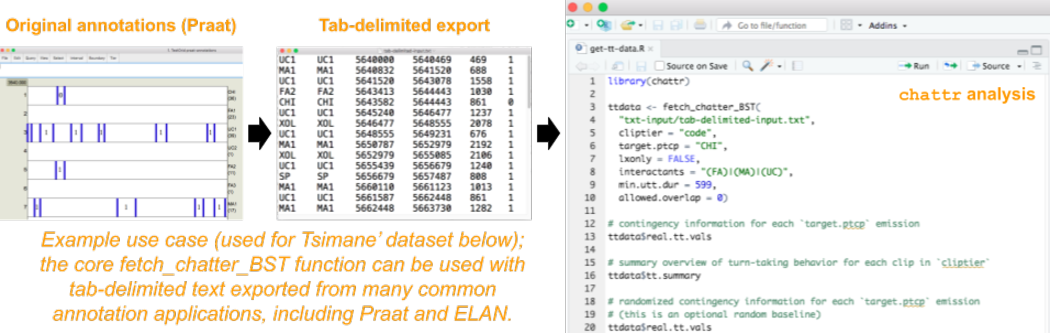
\includegraphics{figs/workflow-1} 

}

\caption[Example workflow for an annotation file using `chattr']{Example workflow for an annotation file using `chattr'.}\label{fig:workflow}
\end{figure*}
\end{CodeChunk}

Beyond LENA, approaches to extracting temporal contingencies have been
much more variable. For example, in studies of adult conversation,
researchers vary in what timing windows qualify as contingent, what
types of contributions count toward turn taking, the modality in which
communication is taking place, in how many interactants are considered
to be involved (or are of interest), and so on, as is suitable to the
research question (e.g., Ten Bosch, Oostdijk, \& Boves, 2005; Fröhlich
et al., 2016; Heldner \& Edlund, 2010; Pika et al., 2018; Roberts,
Torreira, \& Levinson, 2015). These studies, while heterogeneous in data
types and determinants for how and when to count turn-taking exchanges,
have typically been inspired by the same set of core concepts from
conversation analysis, building up significant theoretical common ground
for understanding moment-to-moment processes of interactant
coordination. Much of the work on language development, by contrast, has
inherited the somewhat idiosyncratic concepts and terminology introduced
by the LENA system, leaving a conceptual disjunct between work on
turn-taking behaviors in children, adults, and non-human animals. Given
the various restrictions on existing tools and free variations in
analysis across studies, there is a clear need for a free, flexible, and
theoretically grounded tool that can extract temporal contingencies at
scale; \texttt{chattr} fills this need.

\hypertarget{the-chattr-system}{%
\section{\texorpdfstring{The \texttt{chattr}
system}{The chattr system}}\label{the-chattr-system}}

In brief, \texttt{chattr} is an R package that gives both summary and
detailed data on temporal contingencies in pre-annotated data. To keep
things simple, it has a single core function for each type of input that
it takes: (a) LENA .its files; (b) tab delimited .txt tables with one
production/utterance per row (e.g., exported from Praat, ELAN, etc.,
Figure 2; Wittenburg, Brugman, Russel, Klassmann, \& Sloetjes, 2006;
Boersma \& Weenink, 2021); and (c) .rttm tables, a common output format
used with automated speech diarization systems.\footnote{If interested
  in a fully open-source pipeline for child language environments, try
  Lavechin et al.'s (2021) voice type classifier.} Users can use the
default settings for each function---including limits on the relevant
temporal windows, potential interactants, and which productions are
considered---or can customize as desired. More advanced users can
capitalize on the numerous sub-functions utilized by the core input-type
functions to tailor \texttt{chattr}'s functions to their unique needs.
All settings, output information types, and theoretical background is
thoroughly summarized in the online documentation on the project's
GitHub repository.

\hypertarget{core-concepts}{%
\subsubsection{Core concepts}\label{core-concepts}}

We encourage users to first evaluate how well \texttt{chattr}`s concepts
of 'turn', `transition', and `interactional sequence' fit those of the
study context; our default definitions differ from those typically used
in the language development literature and are restricted compared to
their full (and human conversation-specific) meanings in conversation
analysis (Sacks, Schegloff, \& Jefferson, 1974; Schegloff, 2007). We
briefly summarize these core concepts here (also illustrated in Figure
1). We use the terms `producer' and `recipient'/`addressee' rather than
`speaker' and `listener' to underscore the utility of these concepts
across modalities, species, and interactional contexts:

A \emph{`turn'} comprises one or more closely occurring emissions by the
same producer. That is, a turn can be formed of multiple complete
emissions (e.g., utterances/communicative acts) that may be separated by
pauses in production so long as (a) there is no intervening emission
from another producer and (b) the pause in production is short. An
example of a single-unit turn in English is ``Jane is the one in the
hat.''. An example of a multi-unit turn in English is ``Jane is the one
in the hat {[}pause{]} third from the left.''

A \emph{`turn transition'} occurs when one producer's turn stops and
another producer's turn begins. Every turn transition has a
pre-transition producer and a post-transition producer---these must be
different individuals. The transition \emph{begins} when the first turn
ends and \emph{ends} when the second turn starts. Therefore, if the
second turn starts before the first turn ends, the transition time is
negative (`transitional overlap'). If the second turn starts after the
first turn ends, the transition time is positive (`transitional gap').

An \emph{`interactional sequence'} is an unbroken turn-taking sequence
between the target interactant and one or more of their interactional
partners. Interactional sequences likely index more structurally
complex, engaged interactional behaviors than single turn transitions
do---akin to conversational bouts (or LENA VABs) during which
participants can more substantially build on joint goals.

The \texttt{chattr} default settings are designed for human spontaneous
conversation, including child conversation, which demonstrates fairly
robust timing patterns (with some systematic variation) across the
signed and spoken languages that have been analyzed (Levinson, 2019).
The three most critical default settings are that: (a) up to 2000 ms of
transitional gap or up to 1000 ms of transitional overlap is allowed
between turns, (b) transitions can occur between turns of any duration,
content, and from any potential interactional partner, and (c) when
there are multiple potential prompts or responses (e.g., two
interactants answer a question nearly simultaneously), \texttt{chattr}
picks the production that occurs closest to the present one. Users
interested in emulating LENA's CTC measure with their .its files can use
a specialized function in which the target producer is assumed to be
``CH'' (target child), potential interactants are limited to
``FA''/``MA'' (female and male adult), and analyzed turns contain some
linguistic material.

\hypertarget{example-use-case}{%
\subsubsection{Example use case}\label{example-use-case}}

Suppose that I am interested in investigating how adult turn-taking
varies in a dataset across semi-structured contexts (e.g., during board
game play). I would ensure that the annotations are formatted as
tab-delimited text (e.g., Figure 2). Then I would use the core Basic
Speech Table call \texttt{fetch\_chatter\_BST()} to fetch turn-taking
information. I might also want to, e.g., define a minimum utterance
duration and a more strict temporal window for contingency, as well as
calculate 10 randomized simulations of turn-taking rates to assess the
baseline likelihood contingency:
\texttt{fetch\_chatter\_BST(filename,\ min.utt.dur\ =\ 1500,\ allowed.gap\ =\ 1000,\ allowed.overlap\ =\ 600,\ n.runs\ =\ 10)}.
This call yields detailed tables of detected turn-taking behavior ready
for the author's statistical analysis of choice.

\hypertarget{pilot-analysis}{%
\section{Pilot analysis}\label{pilot-analysis}}

We demonstrate the use of \texttt{chattr} with three child language
environment datasets from unrelated rural Indigenous communities:
specifically, we sanity check \texttt{chattr}`s performance on corpora
for which we have strong a priori hypotheses about basic turn-taking
patterns. The analyzed recordings document children's verbal
interactional patterns over full days at home in understudied and rural
populations, for which use of a tool like LENA would be challenging.
\texttt{Chattr} allows us to examine interactional patterns at scale in
these corpora, evading months of manual annotation that would achieve
the same, and making it easy to do so for both conventional (child-adult
interaction) and non-conventional (child-child interactional) categories
relevant to development in these contexts. The first two corpora,
Tseltal (Mayan; Chiapas, Mexico; N = 10) and Yélî Dnye (isolate; Milne
Bay, Papua New Guinea; N = 10), come from the Casillas HomeBank
repository (Casillas et al., 2017) and were made with near parallel
methods: children under age 3;0 wore an Olympus WS-832/853 audio
recorder at home for 8--11 hours. The third corpus, Tsimane' (Tsimane';
Bolivia; 40 recordings from 27 children) features children under 6;0 who
wore one of multiple recording devices (LENA, Olympus, or USB) at home
for 4--21 hours (Scaff, Stieglitz, Casillas, \& Cristia, n.d.); we focus
here on the subset of those 17 recordings made with LENA (from 13
children). In each dataset we assess the baseline turn-taking rate over
age and the frequency of interactions with other children. For the
Tsimane' corpus can also compare \texttt{chattr} estimates on both LENA
(automated) and manually created annotations of the same recording
minutes. This pilot studies thus test whether previously documented
patterns in these children's linguistic input are recapitulated in their
turn-taking behavior, as detected by \texttt{chattr}.

\hypertarget{study-1.-tseltal-and-yuxe9luxee-dnye}{%
\subsection{Study 1. Tseltal and Yélî
Dnye}\label{study-1.-tseltal-and-yuxe9luxee-dnye}}

We analyze interactional behavior in 20 clips for each recording: 9
randomly selected clips (5 min for Tseltal and 2.5 min for Yélî Dnye), 5
clips manually selected for day-peak turn-taking behavior of the target
child with one or more interactants (each 1 min), 5 clips manually
selected for day-peak vocal activity by the target child (each 1 min),
and one 5-minute expansion on the most active turn-taking/vocal-activity
clip. Each clip was manually annotated for all hearable speech,
including addressee coding (e.g., target-child-directed
vs.~other-directed; see Casillas et al.~(2020b, 2020a)). Despite
documented differences in caregiver-child interactional style, day-long
linguistic input estimates show similar patterns in these two
communities. While female adult speech constitutes the majority of
linguistic input in both communities, Yélî children show a marked
increase in directed speech from other children with age. This pattern
appears more weakly in the Tseltal data. We therefore expected to find
that: (1) turn-taking rates are higher in turn-taking and vocal activity
clips than in random clips, (2) rates are similar between the two
communities, and (3) interactional sequences involving other children
increase with age, particularly for Yélî children.

\begin{CodeChunk}
\begin{figure}[h]

{\centering 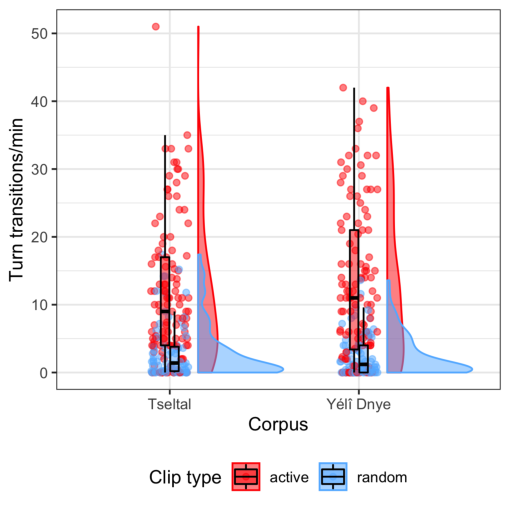
\includegraphics{figs/tseyel.ttr.fig-1} 

}

\caption[Turn transition rate by corpus, divided across manually selected turn-taking/high-vocal-activity clips (red) and random clips (blue)]{Turn transition rate by corpus, divided across manually selected turn-taking/high-vocal-activity clips (red) and random clips (blue).}\label{fig:tseyel.ttr.fig}
\end{figure}
\end{CodeChunk}

\begin{CodeChunk}
\begin{figure}[h!]

{\centering 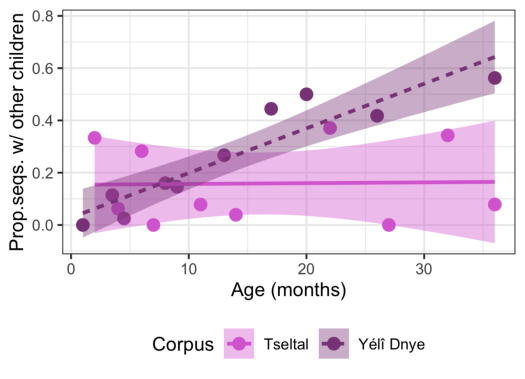
\includegraphics{figs/tseyel.is.fig-1} 

}

\caption[Proportion of interactional sequences involving at least one non-target child across age, by language]{Proportion of interactional sequences involving at least one non-target child across age, by language.}\label{fig:tseyel.is.fig}
\end{figure}
\end{CodeChunk}

\hypertarget{methods}{%
\subsubsection{Methods}\label{methods}}

We use \texttt{fetch\_chatter\_AAS()}, which is specifically designed
for those using the ACLEW\footnote{\href{https://sites.google.com/view/aclewdid/home}{sites.google.com/view/aclewdid/}.}
Annotation Scheme (Casillas, Bergelson, et al., 2017). It allows 2000 ms
of gap and 1000 ms of overlap at turn transitions and searches over all
annotated utterances (any duration, content, and from any speaker). We
limit our analysis to utterances directed exclusively to the target
child. We also indicate the annotated regions by using the
\texttt{cliptier} argument.

\hypertarget{results}{%
\subsubsection{Results}\label{results}}

The mean rate of turn transitions in the Tseltal corpus was 11.8 and 3
transitions per minute for the active (turn taking and vocal activity)
and random clips, respectfully, and 12.8 and 2.4 transitions per minute
for Yélî Dnye. The distribution of turn taking rates across annotated
clips was similar between the two sites (Table 1). A linear mixed
effects regression of transitions per minute with predictors of clip
type, corpus, and their interaction, and a random intercept for child
reveals that random clips indeed have significantly lower transition
rates (B = -8.78, SE = 1.2, t = -7.31). There is no evidence for a
significant difference in rates between languages (t = 0.54) and no
evidence for a clip type-language interaction (t = -0.74).

A second linear mixed effects regression of the proportion of
interactional sequences featuring at least one non-target child with
predictors of age (in months), corpus, and their interaction, and a
random intercept for child reveals that there is indeed a significant
age-by-corpus interaction by which Yélî children show a larger increase
in other-child interactional sequences with age compared to Tseltal
children (B = 0.01, SE = 0.01, t = 2.47). There is no evidence for
simple effects of age (t = 0.2) or language (t = -0.99).

\hypertarget{study-2.-tsimane}{%
\subsection{Study 2. Tsimane'}\label{study-2.-tsimane}}

These Tsimane' recordings were first automatically analyzed with LENA
and then subsequently (and independently) manually annotated in 1-minute
clips every 60 minutes, starting at the 34th minute (min 34-35, min
94-95, min 154-155, etc.; Scaff et al., n.d.). Both annotation types
(LENA and manual) encode (a) when speech was occurring and (b) what type
of speaker produced it (i.e., the target child, a nearby woman/man/other
child, or other) for each of the hand-annotated minutes. Prior analysis
shows comparably low rates of directed speech in these Tsimane' data to
the Tseltal and Yélî Dnye recordings, again with a high proportion of
directed input coming from other children (Scaff et al., n.d.). We
therefore expected to find that: (1) despite their slightly different
operationalizations, turn-taking rates are overall similar to what we
found in the random samples of the other two communities , (2)
turn-taking sequences involving other children are comparable to or more
frequent than those in the random samples of the other two communities,
(3) interactional sequences involving other children increase with age,
and (4) manual and automated speech annotations of the same audio clips
result in similar turn-taking estimates.

\begin{table}[h]
\centering
\begin{tabular}{lll}
  \hline
Corpus & Clip type & mean (sd; range), median \\ 
  \hline
Tseltal & active (manual) & 11.8 (4.8; 4.5-20.1), 12.3 \\ 
  Tseltal & random (manual) & 3 (3.1; 0.4-10.6), 2.3 \\ 
  Yélî Dnye & active (manual) & 12.8 (6.5; 3.9-22.2), 10.8 \\ 
  Yélî Dnye & random (manual) & 2.4 (1.6; 0.5-6), 2.2 \\ 
  Tsimane' & random (LENA) & 3.2 (1.1; 1.2-5.1), 3.1 \\ 
  Tsimane' & random (manual) & 3.2 (1.2; 1.3-6), 3 \\ 
   \hline
\end{tabular}
\end{table}

\begin{CodeChunk}
\begin{figure}[h]

{\centering 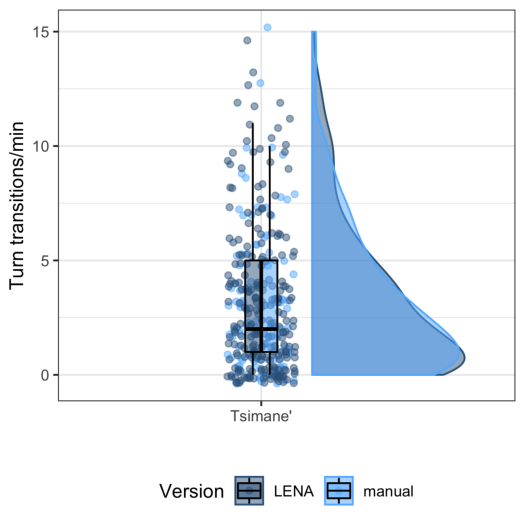
\includegraphics{figs/tsi.ttr.fig-1} 

}

\caption[Turn transition rate by annotation type (LENA automated vs]{Turn transition rate by annotation type (LENA automated vs. manual) in the same audio clips. Clips are a periodic random sample of the daylong recording.}\label{fig:tsi.ttr.fig}
\end{figure}
\end{CodeChunk}

\begin{CodeChunk}
\begin{figure}[h!]

{\centering 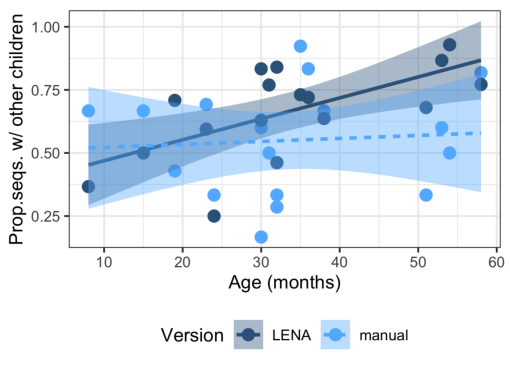
\includegraphics{figs/tsi.is.fig-1} 

}

\caption[Proportion of interactional sequences involving at least one non-target child across age, by annotation type (LENA automated vs]{Proportion of interactional sequences involving at least one non-target child across age, by annotation type (LENA automated vs. manual) in the same audio clips.}\label{fig:tsi.is.fig}
\end{figure}
\end{CodeChunk}

\hypertarget{methods-1}{%
\subsubsection{Methods}\label{methods-1}}

We use \texttt{fetch\_chatter\_BST()} with the manually annotated data,
matching conditions of the call as closely as possible to what can be
compared in the LENA output files, that is: include woman, man, and
other-child speech, both linguistic and non-linguistic, with a minimum
utterance duration of 600ms (the LENA lower limit) and no overlap
allowed (meaningful overlap is not possible in LENA). With the automatic
LENA annotations on the same recordings (the same 1-minute segments) we
adjust the default settings on \texttt{fetch\_chatter\_LENA()} to
reflect these same restrictions.

\hypertarget{results-1}{%
\subsubsection{Results}\label{results-1}}

A linear mixed effects regression of transitions per minute with a fixed
effect of annotation type (LENA vs.~manual) and a random intercept for
child reveals that turn-transition rates are similar between the two
annotation methods (B = -0.09, SE = 0.41, t = -0.23). As expected,
turn-transition rates are similar to what we found in the Tseltal and
Yélî Dnye random clips, at 3.2 transitions per minute, though with fewer
instances of rates above 10/min (Table 1).

A second linear mixed effects regression of the proportion of
interactional sequences featuring at least one non-target child with
predictors of age (in months), annotation type (LENA vs.~manual), and
their interaction, and a random intercept for child reveals that, as
expected, there is a significant increase in other-child interactional
sequences with age (B = 0.01, SE = 0, t = 3.39). There is no evidence
for simple effects of annotation type (t = 0.71) or for an
age-annotation type interaction (t = -1.39).

\hypertarget{contribution-and-next-steps}{%
\section{Contribution and next
steps}\label{contribution-and-next-steps}}

The \texttt{chattr} package allows users to easily implement
theoretically informed contingency analyses on a wide variety of data
types, including both automatically and manually annotated data. The
package is designed for both straightforward (i.e., basic
\texttt{fetch\_chatter} calls) and customized analysis scenarios and
provides detailed outputs that can be merged with other data about the
same recordings. By providing a single tool for analyzing the most
common input formats used for interactional data in psychology, animal
behavior, and speech technology research, \texttt{chattr} aims to help
build theoretical and methodological connections regarding the nature of
contingent behaviors across diverse domains. While \texttt{chattr} has
now been tested on a variety of child language datasets, new
functionality will emerge following user issue-posting and feature
requests. Following the beta stage of development, we will make the
package available on CRAN for easier distribution. A critical next step
will also be the development of tutorial materials to accompany the
documentation, enabling new R users to quickly apply the core functions
to a sampling of common use cases.

\hypertarget{acknowledgements}{%
\section{Acknowledgements}\label{acknowledgements}}

REDACTED

\hypertarget{references}{%
\section{References}\label{references}}

\setlength{\parindent}{-0.1in} 
\setlength{\leftskip}{0.125in}

\noindent

\hypertarget{refs}{}
\leavevmode\hypertarget{ref-PRAAT}{}%
Boersma, P., \& Weenink, D. (2021). Praat: Doing phonetics by computer.
Retrieved from \url{http://www.praat.org}

\leavevmode\hypertarget{ref-casillas2017workflow}{}%
Casillas, M., Bergelson, E., Warlaumont, A. S., Cristia, A., Soderstrom,
M., VanDam, M., \& Sloetjes, H. (2017). A new workflow for
semi-automatized annotations: Tests with long-form naturalistic
recordings of children's language environments. In \emph{Proceedings of
INTERSPEECH 2017} (pp. 2098--2102). Stockholm, Sweden.

\leavevmode\hypertarget{ref-Casillas-HB}{}%
Casillas, M., Brown, P., \& Levinson, S. C. (2017). Casillas HomeBank
corpus. \url{http://doi.org/10.21415/T51X12}

\leavevmode\hypertarget{ref-casillas2020rossel}{}%
Casillas, M., Brown, P., \& Levinson, S. C. (2020a). Early language
experience in a Papuan community. \emph{Journal of Child Language},
1--23.

\leavevmode\hypertarget{ref-casillas2020tseltal}{}%
Casillas, M., Brown, P., \& Levinson, S. C. (2020b). Early language
experience in a Tseltal Mayan village. \emph{Child Development},
\emph{91}(5), 1819--1835.

\leavevmode\hypertarget{ref-cristia2020accuracy}{}%
Cristia, A., Bulgarelli, F., \& Bergelson, E. (2020). Accuracy of the
language environment analysis system segmentation and metrics: A
systematic review. \emph{Journal of Speech, Language, and Hearing
Research}, \emph{63}(4), 1093--1105.

\leavevmode\hypertarget{ref-ferjan2021comparing}{}%
Ferjan Ramírez, N., Hippe, D. S., \& Kuhl, P. K. (2021). Comparing
automatic and manual measures of parent--infant conversational turns: A
word of caution. \emph{Child Development}, 1--10.

\leavevmode\hypertarget{ref-frohlich2016unpeeling}{}%
Fröhlich, M., Kuchenbuch, P., Müller, G., Fruth, B., Furuichi, T.,
Wittig, R. M., \& Pika, S. (2016). Unpeeling the layers of language:
Bonobos and chimpanzees engage in cooperative turn-taking sequences.
\emph{Scientific Reports}, \emph{6}(1), 1--14.

\leavevmode\hypertarget{ref-LENA}{}%
Greenwood, C. R., Thiemann-Bourque, K., Walker, D., Buzhardt, J., \&
Gilkerson, J. (2011). Assessing children's home language environments
using automatic speech recognition technology. \emph{Communication
Disorders Quarterly}, \emph{32}(2), 83--92.

\leavevmode\hypertarget{ref-heldner2010pauses}{}%
Heldner, M., \& Edlund, J. (2010). Pauses, gaps and overlaps in
conversations. \emph{Journal of Phonetics}, \emph{38}(4), 555--568.

\leavevmode\hypertarget{ref-lavechin2021vtc}{}%
Lavechin, M., Bousbib, R., Bredin, H., Dupoux, E., \& Cristia, A.
(2021). An open-source voice type classifier for child-centered daylong
recordings. Retrieved from \url{http://arxiv.org/abs/2005.12656}

\leavevmode\hypertarget{ref-levinson2019interactional}{}%
Levinson, S. C. (2019). Interactional foundations of language: The
interaction engine hypothesis. In \emph{Human language: From genes and
brain to behavior} (pp. 189--200). MIT Press.

\leavevmode\hypertarget{ref-pika2018taking}{}%
Pika, S., Wilkinson, R., Kendrick, K. H., \& Vernes, S. C. (2018).
Taking turns: Bridging the gap between human and animal communication.
\emph{Proceedings of the Royal Society B}, \emph{285}(1880), 20180598.

\leavevmode\hypertarget{ref-roberts2015effects}{}%
Roberts, S. G., Torreira, F., \& Levinson, S. C. (2015). The effects of
processing and sequence organization on the timing of turn taking: A
corpus study. \emph{Frontiers in Psychology}, \emph{6}, 509.

\leavevmode\hypertarget{ref-rodriguez2019you}{}%
Rodríguez-Arauz, G., Ramírez-Esparza, N., García-Sierra, A., Ikizer, E.
G., \& Fernández-Gómez, M. J. (2019). You go before me, please:
Behavioral politeness and interdependent self as markers of simpatía in
Latinas. \emph{Cultural Diversity and Ethnic Minority Psychology},
\emph{25}(3), 379.

\leavevmode\hypertarget{ref-romeo2018beyond}{}%
Romeo, R. R., Leonard, J. A., Robinson, S. T., West, M. R., Mackey, A.
P., Rowe, M. L., \& Gabrieli, J. D. E. (2018). Beyond the
30-million-word gap: Children's conversational exposure is associated
with language-related brain function. \emph{Psychological Science},
\emph{29}(5), 700--710.

\leavevmode\hypertarget{ref-sacks1974simplest}{}%
Sacks, H., Schegloff, E. A., \& Jefferson, G. (1974). A simplest
systematics for the organization of turn taking for conversation. In
\emph{Studies in the organization of conversational interaction} (pp.
7--55). Elsevier.

\leavevmode\hypertarget{ref-scaffIPlanguage}{}%
Scaff, C., Stieglitz, J., Casillas, M., \& Cristia, A. (n.d.). Daylong
audio recordings of young children in a forager-farmer society show low
levels of verbal input with minimal age-related change.

\leavevmode\hypertarget{ref-schegloff2007sequence}{}%
Schegloff, E. A. (2007). \emph{Sequence organization in interaction: A
primer in conversation analysis I} (Vol. 1). Cambridge university press.

\leavevmode\hypertarget{ref-ten2005temporal}{}%
Ten Bosch, L., Oostdijk, N., \& Boves, L. (2005). On temporal aspects of
turn taking in conversational dialogues. \emph{Speech Communication},
\emph{47}(1-2), 80--86.

\leavevmode\hypertarget{ref-ELAN}{}%
Wittenburg, P., Brugman, H., Russel, A., Klassmann, A., \& Sloetjes, H.
(2006). ELAN: A professional framework for multimodality research. In
\emph{Proceedings of the Fifth International Conference on Language
Resources and Evaluation} (pp. 1556--1559).

\bibliographystyle{apacite}


\end{document}
